\documentclass[12pt]{article}

\usepackage[margin=1in]{geometry}
\usepackage[T1]{fontenc}
\usepackage{lmodern}
\usepackage{microtype}
\usepackage{amsmath,amssymb,mathtools}
\usepackage{booktabs}
\usepackage{enumitem}
\usepackage{setspace}
\usepackage{tikz}
\usepackage{hyperref}
\usepackage{xurl}

\hypersetup{
  pdftitle={The Temporal Propagator: Finite-Window Averages, Operator Structure, and Clock-Rate Applications},
  pdfauthor={Light-Meter Physics},
  colorlinks=true,
  linkcolor=black,
  citecolor=black,
  urlcolor=blue
}

\onehalfspacing
\widowpenalty=10000
\clubpenalty=10000

\title{The Temporal Propagator:\\
Finite-Window Averages, Operator Structure, and Clock-Rate Applications}
\author{Light-Meter Physics}
\date{Draft Manuscript}

\begin{document}

\maketitle

\begin{abstract}
This paper develops the Light-Meter Physics use of the term \emph{temporal propagator} as a pair of finite-window averages acting on a specified time-dependent signal. Starting from the integral definitions, it derives the translation-operator forms, a derivative expansion with a finite-order remainder bound, an exact even--odd decomposition, the Fourier response, and the triangular kernel obtained by composing the two windows. The averaging operators have sinc zeros and therefore do not possess a universal inverse on signal spaces containing the corresponding modes. A separate application expresses a static-spacetime clock-rate comparison as a path average of the inward field. That application is an exact rewriting of the static lapse-gradient identity, not a new gravitational law. Throughout, the paper distinguishes mathematical identities from regularity assumptions and physical modeling choices. The temporal propagator is project terminology for finite-window averaging; it is not a Green function, a field equation, or evidence for a physical propagation mechanism.
\end{abstract}

\noindent\textbf{Keywords:} finite-window average, translation operator, sinc response, clock-rate comparison, static spacetime, lapse

\section{Introduction}

A finite-duration average is a simple way to map a time-dependent signal to a smoothed signal. In the Light-Meter Physics materials, this construction is called the \emph{temporal propagator}. The name is used here only for the averaging operators defined below. It does not mean a standard propagation kernel, an electromagnetic Green function, or a mechanism that transports a physical signal through time.

The aim is to give the construction a self-contained mathematical treatment before discussing an application. We define future- and past-sampling windows of equal duration, derive their exact operator forms, determine their even and odd parts, and examine their behavior on Fourier modes. We also derive the response of two windows composed in succession and identify signal classes on which inversion fails. A final application rewrites the exact static clock-rate comparison between two locations as a finite path average.

Three levels of claim will be kept separate. The integral identities follow from the definitions under local integrability. The derivative series and its error estimate require additional differentiability, and convergence of an infinite Taylor series requires more than smoothness. The clock-rate application assumes a specified static geometry and a chosen spatial path; it does not follow from the averaging operator alone. A structural comparison with the paired decompositions discussed in Manuscript 21 is mathematical only \cite{LMP21}.

\section{Definitions, domain, and notation}

Let $g$ be a real- or complex-valued, locally integrable signal on an interval that contains the sampling windows. Choose a positive duration
\begin{equation}
  \tau_L\equiv\frac{L}{c}>0,
  \label{eq:tau-L}
\end{equation}
where $L$ is a specified length and $c$ is the speed of light. For a specified time coordinate $t$, define
\begin{align}
  \mathcal{P}_{+}[g](t)
  &\equiv\frac{1}{\tau_L}\int_0^{\tau_L}g(t+u)\,\mathrm{d}u,
  \label{eq:window-definitions}\\
  \mathcal{P}_{-}[g](t)
  &\equiv\frac{1}{\tau_L}\int_0^{\tau_L}g(t-u)\,\mathrm{d}u.\notag
\end{align}
The corresponding intervals are $[t,t+\tau_L]$ for $\mathcal{P}_{+}$ and $[t-\tau_L,t]$ for $\mathcal{P}_{-}$. A change of integration variable gives the equivalent forms
\begin{equation}
  \mathcal{P}_{+}[g](t)
  =\frac{1}{\tau_L}\int_t^{t+\tau_L}g(s)\,\mathrm{d}s,
  \qquad
  \mathcal{P}_{-}[g](t)
  =\frac{1}{\tau_L}\int_{t-\tau_L}^{t}g(s)\,\mathrm{d}s.
  \label{eq:shifted-integrals}
\end{equation}
Both operators preserve constant inputs. Their outputs have the same physical units as $g$ because the integral is divided by an interval of time. The duration $\tau_L$ is a chosen window length; writing it as $L/c$ does not by itself establish that the window is an actual signal-travel time.

The subscripts indicate which values of the input signal are sampled relative to $t$. The past-sampling operator $\mathcal{P}_{-}$ uses values up to the present time; the future-sampling operator $\mathcal{P}_{+}$ requires values later than $t$, a prediction, or delayed reporting. These terms do not denote retarded or advanced boundary conditions for a field equation.

\section{Translation-operator form}

Let $D\equiv\mathrm{d}/\mathrm{d}t$ and define the translation $T_u$ on signals whose domain contains $t+u$ by
\begin{equation}
  (T_ug)(t)\equiv g(t+u).
\end{equation}
For a sufficiently regular $g$, $T_u=e^{uD}$, so $g(t-u)=e^{-uD}g(t)$. Substituting these translations into Eq.~\eqref{eq:window-definitions} gives
\begin{align}
  \mathcal{P}_{+}
  &=\frac{1}{\tau_L}\int_0^{\tau_L}e^{uD}\,\mathrm{d}u
   =\frac{e^{\tau_LD}-1}{\tau_LD},
  \label{eq:operator-plus}\\
  \mathcal{P}_{-}
  &=\frac{1}{\tau_L}\int_0^{\tau_L}e^{-uD}\,\mathrm{d}u
   =\frac{1-e^{-\tau_LD}}{\tau_LD}.
  \label{eq:operator-minus}
\end{align}
These quotients are shorthand for entire functions of the translation generator. In particular, for a scalar argument $z$, define
\begin{equation}
  \varphi_{+}(z)\equiv\int_0^1e^{sz}\,\mathrm{d}s
  =\begin{cases}(e^z-1)/z,&z\ne0,\\1,&z=0,\end{cases}
  \qquad
  \varphi_{-}(z)\equiv\int_0^1e^{-sz}\,\mathrm{d}s
  =\begin{cases}(1-e^{-z})/z,&z\ne0,\\1,&z=0.\end{cases}
  \label{eq:entire-window-functions}
\end{equation}
Thus $\mathcal{P}_{\pm}=\varphi_{\pm}(\tau_LD)$ whenever the translation-operator notation is defined. The apparent singularities at $D=0$ are removable; both operators reduce to the identity on constant functions. This construction does not require an inverse derivative $D^{-1}$ or an integration constant. The scalar functions are entire, but that fact alone does not guarantee that their derivative power series converge to their action on every smooth signal; the signal-level Taylor expansion below uses an explicit uniform-convergence hypothesis. The integral definitions remain primary and apply to locally integrable signals.

Changing the sampled interval also shows directly that
\begin{equation}
  \mathcal{P}_{-}[g](t)=\mathcal{P}_{+}[g](t-\tau_L),
  \qquad
  \mathcal{P}_{-}=e^{-\tau_LD}\mathcal{P}_{+}.
  \label{eq:translation-relation}
\end{equation}
This is a translation relation, not an inverse relation: in general $\mathcal{P}_{-}\ne\mathcal{P}_{+}^{-1}$.

\section{Derivative expansion and remainder bound}\label{sec:derivative-expansion}

Suppose the Taylor series of $g$ about $t$ converges uniformly to $g$ throughout $[t-\tau_L,t+\tau_L]$. Expand $g(t\pm u)$ and integrate term by term. The coefficient of the $k$th derivative follows from
\begin{equation}
  \frac{1}{\tau_L}\int_0^{\tau_L}\frac{(\pm u)^k}{k!}\,\mathrm{d}u
  =\frac{(\pm\tau_L)^k}{(k+1)!}.
\end{equation}
Consequently,
\begin{equation}
  \mathcal{P}_{\pm}[g](t)
  =\sum_{k=0}^{\infty}\frac{(\pm\tau_L)^k}{(k+1)!}g^{(k)}(t)
  =g(t)\pm\frac{\tau_L}{2}g'(t)
   +\frac{\tau_L^2}{6}g''(t)
   \pm\frac{\tau_L^3}{24}g'''(t)+\cdots.
  \label{eq:derivative-expansion}
\end{equation}
Each derivative is with respect to the specified coordinate $t$. If $g$ is a signed acceleration component in a fixed inertial basis and $t$ is that frame's time coordinate, the first derivatives can be called jerk, snap, and crackle. For a generic signal, they are simply time derivatives; they are not automatically proper-time derivatives or covariant derivatives.

An infinite series is not needed for a controlled finite-order approximation. Let $n\geq0$, suppose $g\in C^{n+1}$ on the interval containing both windows, and set
\begin{equation}
  M_{n+1}\equiv\sup_{|v-t|\leq\tau_L}|g^{(n+1)}(v)|.
  \label{eq:derivative-bound-definition}
\end{equation}
Taylor's theorem gives, for $0\leq u\leq\tau_L$ and either sign,
\begin{equation}
  g(t\pm u)
  =\sum_{k=0}^{n}\frac{(\pm u)^k}{k!}g^{(k)}(t)+R_{n+1,\pm}(t,u),
  \qquad
  |R_{n+1,\pm}(t,u)|\leq\frac{M_{n+1}u^{n+1}}{(n+1)!}.
  \label{eq:taylor-remainder-pointwise}
\end{equation}
Averaging the remainder and integrating the power of $u$ yields
\begin{equation}
  \left|
  \mathcal{P}_{\pm}[g](t)
  -\sum_{k=0}^{n}\frac{(\pm\tau_L)^k}{(k+1)!}g^{(k)}(t)
  \right|
  \leq\frac{M_{n+1}\tau_L^{n+1}}{(n+2)!}.
  \label{eq:derivative-remainder-bound}
\end{equation}
The integral averages need only local integrability, whereas Eq.~\eqref{eq:derivative-remainder-bound} requires the stated smoothness. Even $C^{\infty}$ regularity alone does not guarantee convergence of the infinite Taylor series to $g$; the uniform-convergence condition above is one sufficient hypothesis for Eq.~\eqref{eq:derivative-expansion}.

\section{Exact even--odd decomposition}

Define the symmetric and antisymmetric combinations of the window operators by
\begin{equation}
  \mathcal{E}\equiv\frac{\mathcal{P}_{+}+\mathcal{P}_{-}}{2},
  \qquad
  \mathcal{O}\equiv\frac{\mathcal{P}_{+}-\mathcal{P}_{-}}{2}.
  \label{eq:even-odd-definitions}
\end{equation}
Adding the two integral definitions gives the centered average over a total interval of duration $2\tau_L$; subtracting gives the difference of the two one-sided averages:
\begin{align}
  \mathcal{E}[g](t)
  &=\frac{1}{2\tau_L}\int_{-\tau_L}^{\tau_L}g(t+u)\,\mathrm{d}u,
  \label{eq:even-integral}\\
  \mathcal{O}[g](t)
  &=\frac{1}{2\tau_L}\int_0^{\tau_L}
    \bigl[g(t+u)-g(t-u)\bigr]\,\mathrm{d}u.
  \label{eq:odd-integral}
\end{align}
Using Eqs.~\eqref{eq:operator-plus}--\eqref{eq:operator-minus} and the hyperbolic-function identities gives the equivalent operator expressions
\begin{equation}
  \mathcal{E}=\frac{\sinh(\tau_LD)}{\tau_LD},
  \qquad
  \mathcal{O}=\frac{\cosh(\tau_LD)-1}{\tau_LD}.
  \label{eq:hyperbolic-split}
\end{equation}
The values at $D=0$ are again defined by continuity. Under the same uniform-convergence hypothesis as in Sec.~\ref{sec:derivative-expansion}, expanding the hyperbolic functions and integrating the even and odd Taylor terms gives
\begin{align}
  \mathcal{E}[g](t)
  &=g(t)+\frac{\tau_L^2}{6}g''(t)
    +\frac{\tau_L^4}{120}g^{(4)}(t)+\cdots,
  \label{eq:even-series}\\
  \mathcal{O}[g](t)
  &=\frac{\tau_L}{2}g'(t)
    +\frac{\tau_L^3}{24}g'''(t)
    +\frac{\tau_L^5}{720}g^{(5)}(t)+\cdots.
  \label{eq:odd-series}
\end{align}
The even operator contains even derivatives and the odd operator contains odd derivatives. This is a parity split of a paired set of one-dimensional averaging operators; it is not a field decomposition and does not represent an absorber response.

\section{Frequency response}

Adopt the Fourier-mode convention $g(t)=e^{i\omega t}$, so $D$ acts on the mode as multiplication by $i\omega$. Applying the integrals directly gives the transfer functions
\begin{align}
  H_{+}(\omega)
  &\equiv\frac{1}{\tau_L}\int_0^{\tau_L}e^{i\omega u}\,\mathrm{d}u
   =e^{i\omega\tau_L/2}
    \operatorname{sinc}\!\left(\frac{\omega\tau_L}{2}\right),
  \label{eq:transfer-plus}\\
  H_{-}(\omega)
  &\equiv\frac{1}{\tau_L}\int_0^{\tau_L}e^{-i\omega u}\,\mathrm{d}u
   =e^{-i\omega\tau_L/2}
    \operatorname{sinc}\!\left(\frac{\omega\tau_L}{2}\right),
  \label{eq:transfer-minus}
\end{align}
where
\begin{equation}
  \operatorname{sinc}(z)\equiv\frac{\sin z}{z},
  \qquad \operatorname{sinc}(0)\equiv1.
  \label{eq:sinc-definition}
\end{equation}
The phase factors locate the centers of the future and past windows at $t+\tau_L/2$ and $t-\tau_L/2$, respectively. The sinc factor is the averaging envelope, so $|H_{\pm}(\omega)|=|\operatorname{sinc}(\omega\tau_L/2)|$. Both responses vanish at
\begin{equation}
  \omega\tau_L=2\pi n,
  \qquad n\in\mathbb{Z}\setminus\{0\},
  \label{eq:sinc-zeros}
\end{equation}
while the zero-frequency, constant mode passes unchanged.

Writing $z=\omega\tau_L/2$, the even and odd transfer functions are
\begin{equation}
  H_{\mathcal E}(\omega)=\cos z\,\operatorname{sinc}(z),
  \qquad
  H_{\mathcal O}(\omega)=i\sin z\,\operatorname{sinc}(z).
  \label{eq:even-odd-transfer}
\end{equation}
For real inputs, the even response is real and even in $\omega$, while the odd response is imaginary and odd. These are the frequency-domain forms of the paired-window parity decomposition.

\section{Composition, null modes, and inversion limits}

The composition of two windows has a useful exact kernel. Applying the past window to the output of the future window gives
\begin{align}
  (\mathcal{P}_{-}\mathcal{P}_{+})[g](t)
  &=\frac{1}{\tau_L^2}
    \int_0^{\tau_L}\!\int_0^{\tau_L}
      g(t-u+v)\,\mathrm{d}v\,\mathrm{d}u \\
  &=\frac{1}{\tau_L}\int_{-\tau_L}^{\tau_L}
    \left(1-\frac{|w|}{\tau_L}\right)g(t+w)\,\mathrm{d}w.
  \label{eq:triangular-composition}
\end{align}
For fixed $w=v-u$, the allowed interval of $u$ in the square $[0,\tau_L]^2$ has length $\tau_L-|w|$ for $w\in[-\tau_L,\tau_L]$ and is empty otherwise. The change of variables $(u,v)\mapsto(u,w)$ has unit Jacobian, so dividing this interval length by $\tau_L^2$ gives the normalized triangular kernel
\begin{equation}
  K_{\mathrm{comp}}(w)
  =\frac{1}{\tau_L}\left(1-\frac{|w|}{\tau_L}\right)
    \mathbf{1}_{[-\tau_L,\tau_L]}(w),
  \qquad
  \int_{-\tau_L}^{\tau_L}K_{\mathrm{comp}}(w)\,\mathrm{d}w=1.
  \label{eq:triangular-kernel}
\end{equation}
This is the convolution of the two rectangular window kernels. Its Fourier multiplier is the product of Eqs.~\eqref{eq:transfer-plus} and \eqref{eq:transfer-minus}:
\begin{equation}
  H_{\mathrm{comp}}(\omega)
  =H_{-}(\omega)H_{+}(\omega)
  =\operatorname{sinc}^{2}\!\left(\frac{\omega\tau_L}{2}\right).
  \label{eq:composition-response}
\end{equation}

Figure~\ref{fig:window-kernels} illustrates these profiles. The kernels here use the sampled-shift convention $g(t+w)$; in the conventional convolution form $\int K(w)g(t-w)\,\mathrm{d}w$, each one-sided rectangle is reflected, while the centered rectangle and the even triangular kernel are unchanged.

\begin{figure}[ht]
  \centering
  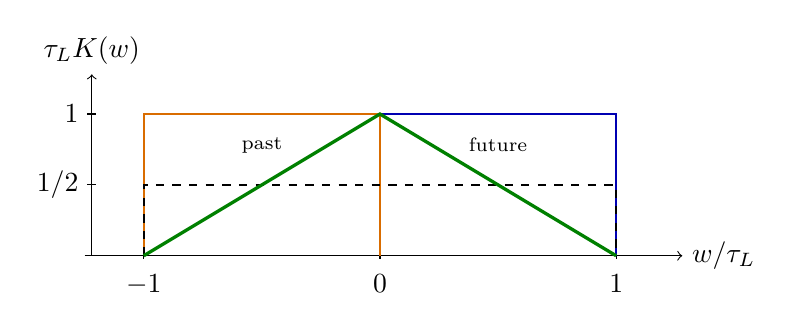
\begin{tikzpicture}[x=3.0cm,y=1.8cm]
    \draw[->] (-1.25,0) -- (1.28,0) node[right] {$w/\tau_L$};
    \draw[->] (-1.22,0) -- (-1.22,1.28) node[above] {$\tau_L K(w)$};
    \foreach \x/\lab in {-1/$-1$,0/$0$,1/$1$} {
      \draw (\x,0.025) -- (\x,-0.025) node[below=2pt] {\lab};
    }
    \draw (-1.24,0.5) -- (-1.20,0.5) node[left=3pt] {$1/2$};
    \draw (-1.24,1) -- (-1.20,1) node[left=3pt] {$1$};
    \draw[blue!70!black,thick] (0,0) -- (0,1) -- (1,1) -- (1,0);
    \draw[orange!85!black,thick] (-1,0) -- (-1,1) -- (0,1) -- (0,0);
    \draw[black,dashed,thick] (-1,0) -- (-1,0.5) -- (1,0.5) -- (1,0);
    \draw[green!50!black,very thick] (-1,0) -- (0,1) -- (1,0);
    \node[font=\scriptsize] at (-0.5,0.78) {past};
    \node[font=\scriptsize] at (0.5,0.78) {future};
  \end{tikzpicture}
  \caption{Normalized kernels as functions of the dimensionless shift $w/\tau_L$, using the sampled-shift convention $g(t+w)$. Past rectangle (orange), future rectangle (blue), centered rectangle (black dashed), and composition triangle (green); the labels distinguish the one-sided plateaus in grayscale. The future and past windows are rectangular kernels on $[0,\tau_L]$ and $[-\tau_L,0]$. Their half-sum is the centered rectangle of height $1/(2\tau_L)$, and their composition is the unit-area triangular kernel of Eq.~\eqref{eq:triangular-kernel}. The vertical axis displays $\tau_L K(w)$, so each plotted kernel has unit area in the dimensionless coordinate. In the conventional $g(t-w)$ convolution convention the one-sided rectangles are reflected.}
  \label{fig:window-kernels}
\end{figure}

The sinc zeros prevent a universal inverse on signal classes that contain the corresponding modes. For example, let $g(t)=A\cos(2\pi t/\tau_L+\phi)$ with $A\ne0$. Each window covers exactly one period, hence
\begin{equation}
  \mathcal{P}_{+}[g](t)
  =\frac{1}{\tau_L}\int_t^{t+\tau_L}g(s)\,\mathrm{d}s=0,
  \qquad
  \mathcal{P}_{-}[g](t)
  =\frac{1}{\tau_L}\int_{t-\tau_L}^{t}g(s)\,\mathrm{d}s=0.
  \label{eq:zero-mode-example}
\end{equation}
Thus a nonzero periodic signal is mapped to zero, and its amplitude and phase cannot be recovered from either average alone. More generally, on spaces of continuous or square-integrable $\tau_L$-periodic signals, all mean-zero components are removed by either one-period average. Consequently neither window has an inverse on those spaces.

This statement is domain-dependent. On $L^2(\mathbb{R})$, $H_{\pm}$ vanish only at discrete frequencies and hence are nonzero almost everywhere. Plancherel's theorem implies $H_{\pm}\widehat{g}=0$ only for $g=0$, so both windows are injective; their inverses on their ranges are unbounded since $\operatorname*{ess\,inf}_{\omega\in\mathbb{R}}|H_{\pm}(\omega)|=0$. For $L^2$ signals with spectrum in a measurable set $S$, a bounded inverse exists exactly when $\operatorname*{ess\,inf}_{\omega\in S}|H_{\pm}(\omega)|>0$; any closed band strictly inside $|\omega|<2\pi/\tau_L$ satisfies this. Excluding zeros alone is insufficient, since gains can approach zero and sinc decays at high frequency. Composition squares the gain, magnifying inverse noise. Translation between windows does not restore lost information.

\section{Worked checks}

Several elementary inputs check the normalization and coefficients directly.

\paragraph{Constant signal.}
For $g(t)=a$, Eqs.~\eqref{eq:window-definitions} give $\mathcal{P}_{+}[g]=\mathcal{P}_{-}[g]=a$. The zero-frequency response is unity.

\paragraph{Affine signal.}
For $g(t)=a+bt$, direct integration gives the exact relations
\begin{equation}
  \mathcal{P}_{\pm}[g](t)=a+b\left(t\pm\frac{\tau_L}{2}\right),
  \qquad
  \mathcal{E}[g](t)=g(t),
  \qquad
  \mathcal{O}[g](t)=\frac{b\tau_L}{2}.
  \label{eq:affine-check}
\end{equation}
This verifies the leading odd term and shows that the derivative expansion terminates for an affine input.

\paragraph{Quadratic signal.}
For $g(t)=a+bt+qt^2$, integration yields
\begin{equation}
  \mathcal{P}_{\pm}[g](t)
  =a+b\left(t\pm\frac{\tau_L}{2}\right)
   +q\left(t^2\pm t\tau_L+\frac{\tau_L^2}{3}\right).
  \label{eq:quadratic-check}
\end{equation}
Since $g''(t)=2q$, the even correction in Eq.~\eqref{eq:derivative-expansion} is $\tau_L^2g''/6=q\tau_L^2/3$, in agreement with the exact average.

\paragraph{Sinusoidal signal.}
For $g(t)=A\cos(\omega t+\phi)$ with $A\geq0$, set $z\equiv\omega\tau_L/2$. Direct averaging gives
\begin{equation}
  \mathcal{P}_{\pm}[A\cos(\omega t+\phi)]
  =A\operatorname{sinc}(z)\cos(\omega t+\phi\pm z).
\end{equation}
The output amplitude is $A|\operatorname{sinc}(z)|$. Relative to the input, its phase shift is $\pm z$ when $\operatorname{sinc}(z)>0$ and $\pm z+\pi$ modulo $2\pi$ when $\operatorname{sinc}(z)<0$; at a sinc zero the output vanishes and its phase is undefined. At $\omega\tau_L=3\pi$, $z=3\pi/2$ and $\operatorname{sinc}(z)=-2/(3\pi)$, making the additional $\pi$ phase essential. At $\omega=2\pi/\tau_L$, the input remains nonzero while both averages vanish, as shown in Eq.~\eqref{eq:zero-mode-example}; this explicitly demonstrates the associated inverse problem.

\section{Conditional application: static clock-rate comparison}

\subsection{Static lapse and endpoint identity}

Consider a static region with metric
\begin{equation}
  \mathrm{d}s^2=-\alpha(\mathbf{x})^2c^2\mathrm{d}t^2
  +h_{ij}(\mathbf{x})\,\mathrm{d}x^i\mathrm{d}x^j,
  \qquad \alpha>0,
  \label{eq:static-metric}
\end{equation}
where $t$ is the chosen static coordinate time and $h_{ij}$ is the spatial metric on a constant-$t$ slice. A static observer has fixed spatial coordinates, so its proper time obeys $\mathrm{d}\tau=\alpha\,\mathrm{d}t$. In accordance with the project notation, define its dimensionless reciprocal rate and the static clock potential by
\begin{equation}
  \delta\tau_{\mathrm{static}}\equiv\frac{\mathrm{d}t}{\mathrm{d}\tau}
  =\frac{1}{\alpha},
  \qquad
  \psi\equiv\ln\delta\tau_{\mathrm{static}}=-\ln\alpha.
  \label{eq:static-rate-potential}
\end{equation}
The symbol $\delta\tau_{\mathrm{static}}$ is a dimensionless rate ratio, not an elapsed proper-time interval. The reference normalization of $t$ should be stated when numerical rate ratios are compared. Under a constant rescaling $t'=kt$ with $k>0$, the lapse and reciprocal rate become $\alpha'=\alpha/k$ and $\delta\tau'_{\mathrm{static}}=k\delta\tau_{\mathrm{static}}$. Individual values depend on this normalization, but the endpoint ratio $\delta\tau_{\mathrm{static},2}/\delta\tau_{\mathrm{static},1}=\alpha_1/\alpha_2$ in Eq.~\eqref{eq:static-endpoint-identity} is invariant.

Let $\nabla_{\mathrm{proper}}$ denote the spatial gradient formed with $h_{ij}$ and measured per unit proper distance. The proper acceleration required to hold a static position is $\mathbf{a}_{\mathrm{hold}}=c^2\nabla_{\mathrm{proper}}\ln\alpha$. Define the inward field for the static observer family as its negative:
\begin{equation}
  \mathbf{g}_{\mathrm{in}}
  \equiv-\mathbf{a}_{\mathrm{hold}}
  =-c^2\nabla_{\mathrm{proper}}\ln\alpha
  =c^2\nabla_{\mathrm{proper}}\ln\delta\tau_{\mathrm{static}}.
  \label{eq:static-field-gradient}
\end{equation}
This is a kinematic identity for static observers, not a formula for the coordinate acceleration of an arbitrary moving body \cite{LMP6,Wald,SantiagoVisser}. It follows from the acceleration of the normalized static Killing flow and does not require introducing a new gravitational field.

For a directed path $C:1\to2$ within the static region, integrate Eq.~\eqref{eq:static-field-gradient} along the proper spatial line element $\mathrm{d}\boldsymbol{\ell}$:
\begin{equation}
  \Delta\psi\equiv\psi_2-\psi_1
  =\ln\!\left(\frac{\delta\tau_{\mathrm{static},2}}
                         {\delta\tau_{\mathrm{static},1}}\right)
  =\frac{1}{c^2}\int_C\mathbf{g}_{\mathrm{in}}
    \cdot\mathrm{d}\boldsymbol{\ell},
  \qquad
  \frac{\delta\tau_{\mathrm{static},2}}
       {\delta\tau_{\mathrm{static},1}}=e^{\Delta\psi}.
  \label{eq:static-endpoint-identity}
\end{equation}
The integral depends only on its endpoints because its integrand is a gradient. Reversing the path reverses the sign of $\Delta\psi$.

\subsection{Schwarzschild exterior check}

For the vacuum exterior of a spherical, nonrotating body of mass $M$, the Schwarzschild line element is \cite{Schwarzschild,Wald}
\begin{equation}
  \mathrm{d}s^2
  =-\left(1-\frac{r_s}{r}\right)c^2\mathrm{d}t^2
   +\left(1-\frac{r_s}{r}\right)^{-1}\mathrm{d}r^2
   +r^2\mathrm{d}\Omega^2,
  \qquad
  r_s\equiv\frac{2GM}{c^2}.
  \label{eq:schwarzschild-metric}
\end{equation}
Its lapse and static reciprocal rate are
\begin{equation}
  \alpha(r)=\sqrt{1-\frac{r_s}{r}},
  \qquad
  \delta\tau_{\mathrm{static}}(r)
  =\left(1-\frac{r_s}{r}\right)^{-1/2}.
  \label{eq:schwarzschild-rate}
\end{equation}
Here $t$ is the standard Schwarzschild time, normalized so that $\alpha\to1$ as $r\to\infty$. The example applies to radii in the vacuum exterior: for a black hole, $r>r_s$; for a material source of radius $R_{\mathrm{source}}$, take $r>R_{\mathrm{source}}$ as well as $r>r_s$. Along an outward radial line at fixed $t$, with $\mathrm{d}r>0$, the proper spatial distance is
\begin{equation}
  \mathrm{d}\ell=\frac{\mathrm{d}r}{\alpha(r)}.
  \label{eq:schwarzschild-proper-distance}
\end{equation}
The proper radial gradient, not the coordinate derivative by itself, gives
\begin{equation}
  \mathbf{g}_{\mathrm{in}}(r)
  =-\frac{GM}{r^2\alpha(r)}\,\hat{\mathbf r},
  \label{eq:schwarzschild-inward-field}
\end{equation}
where $\hat{\mathbf r}$ points outward. For two allowed radii $r_2>r_1$, the endpoint comparison is
\begin{align}
  \Delta\psi
  &=\ln\!\left(
    \frac{\delta\tau_{\mathrm{static}}(r_2)}
         {\delta\tau_{\mathrm{static}}(r_1)}\right) \\
  &=\ln\!\left(\frac{\alpha(r_1)}{\alpha(r_2)}\right)
   =\frac{1}{2}\ln\!\left[
     \frac{1-r_s/r_1}{1-r_s/r_2}\right]
   <0.
  \label{eq:schwarzschild-clock-ratio}
\end{align}
The negative sign agrees with the integral in Eq.~\eqref{eq:static-endpoint-identity}: $\mathbf{g}_{\mathrm{in}}$ points inward, opposite the outward proper line element. The higher static clock has a larger proper-time rate $\mathrm{d}\tau/\mathrm{d}t=\alpha$, while its reciprocal rate $\delta\tau_{\mathrm{static}}$ is smaller.

As a numerical check, take $r_1=2r_s$ and $r_2=4r_s$. Then
\begin{equation}
  \begin{aligned}
    \Delta\psi&=\frac{1}{2}\ln\!\left(\frac{2}{3}\right)=-0.2027325541,\\
    \frac{\delta\tau_{\mathrm{static},2}}{\delta\tau_{\mathrm{static},1}}&=\sqrt{\frac{2}{3}},\\
    \frac{(\mathrm{d}\tau/\mathrm{d}t)_2}{(\mathrm{d}\tau/\mathrm{d}t)_1}&=\frac{\alpha_2}{\alpha_1}=\sqrt{\frac{3}{2}}.
  \end{aligned}
\end{equation}

In the weak-field limit, $\alpha\simeq1+\Phi/c^2$ and $\mathbf{g}_{\mathrm{N}}=-\nabla\Phi$, so the same exact relation reduces to
\begin{equation}
  \Delta\psi\simeq-\frac{\Phi_2-\Phi_1}{c^2}
  =\frac{1}{c^2}\int_1^2\mathbf{g}_{\mathrm{N}}
    \cdot\mathrm{d}\boldsymbol{\ell}.
  \label{eq:weak-field-clock-comparison}
\end{equation}
This is an approximation to the static comparison, not a replacement for the exact lapse relation in a strong field.

\subsection{Path-window representation}

The static endpoint identity can be written as a window average without identifying path position with coordinate time. Parametrize $C$ by proper arclength $\ell\in[0,L]$, let $\hat{\mathbf n}(\ell)$ be its directed unit tangent, and define
\begin{equation}
  u\equiv\frac{\ell}{c},
  \qquad
  \tau_L\equiv\frac{L}{c},
  \qquad
  g_C(u)\equiv\mathbf{g}_{\mathrm{in}}\!\left(\mathbf{x}(cu)\right)
    \cdot\hat{\mathbf n}(cu).
  \label{eq:path-field-profile}
\end{equation}
Substituting $\ell=cu$ into Eq.~\eqref{eq:static-endpoint-identity} gives
\begin{align}
  \Delta\psi
  &=\frac{1}{c^2}\int_0^L
      \mathbf{g}_{\mathrm{in}}\!\left(\mathbf{x}(\ell)\right)
      \cdot\hat{\mathbf n}(\ell)\,\mathrm{d}\ell \\
  &=\frac{1}{c}\int_0^{\tau_L}g_C(u)\,\mathrm{d}u \\
  &=\frac{L}{c^2}\mathcal{P}_{+}^{(u)}[g_C](0)
   =\frac{L}{c^2}\mathcal{P}_{-}^{(u)}[g_C](\tau_L).
  \label{eq:path-window-map}
\end{align}
Here $\mathcal{P}_{\pm}^{(u)}$ means that the window operator acts on the parameter $u$ with duration $\tau_L$. The dimensions are consistent: $g_C$ is an acceleration, $c^{-1}\int g_C\,\mathrm{d}u$ is dimensionless, and $L/c^2$ times its average is also dimensionless. Path reversal reverses both the tangent and the order of sampling. If $C^{-1}$ is parameterized from endpoint 2 back to endpoint 1, its profile is
\begin{equation}
  g_{C^{-1}}(u)=-g_C(\tau_L-u).
\end{equation}
Thus, with $v=\tau_L-u$,
\begin{align*}
  \Delta\psi_{C^{-1}}
  &=\frac{1}{c}\int_0^{\tau_L}g_{C^{-1}}(u)\,\mathrm{d}u
   =-\frac{1}{c}\int_0^{\tau_L}g_C(\tau_L-u)\,\mathrm{d}u \\
  &=-\frac{1}{c}\int_0^{\tau_L}g_C(v)\,\mathrm{d}v
   =-\Delta\psi_C.
\end{align*}
For a radial path of arbitrary orientation, the unsigned proper arclength is $\mathrm{d}\ell=|\mathrm{d}r|/\alpha$; orientation is carried by the directed tangent or vector line element.

The parameter $u=\ell/c$ is a convenient time-dimensioned path parameter, not generally the coordinate travel time of a photon. For a null ray in Eq.~\eqref{eq:static-metric}, its spatial proper length instead obeys $\mathrm{d}\ell=c\alpha\,\mathrm{d}t$. Accordingly, Eq.~\eqref{eq:path-window-map} repackages a known static clock comparison; it does not infer the geometry from an arbitrary acceleration history. Derivatives of $g_C$ with respect to $u$, if used, describe variation along this chosen path parameter and should not automatically be called jerk or snap.

\section{Interpretation and limitations}

The window algebra has three distinct mathematical descriptions: exact integrals for locally integrable inputs, Taylor expansions under suitable convergence hypotheses, and Fourier multipliers for modes or signals whose transform representation is valid. These descriptions are equivalent where their respective hypotheses hold, but their assumptions should not be collapsed. In particular, a finite-order Taylor estimate is not a claim that the infinite derivative series converges.

Manuscript 21 compares future-/past-sampling windows with the retarded/advanced pair in Wheeler--Feynman theory. The only point of contact is the formal organization into paired symmetric and antisymmetric parts. Green functions encode spacetime support and field equations; the operators here average a one-dimensional time history. Neither the window identities nor the triangular composition kernel supplies an absorber response or derives radiation reaction \cite{LMP21}. For clarity, \emph{retarded} and \emph{advanced} are reserved here for Green functions and boundary conditions, while $\mathcal{P}_{\pm}$ are called future- and past-sampling averages.

The static clock-rate application is logically separate. Its endpoint identity requires static observers, a static metric with a specified lapse, a chosen reference time, and a directed path. The exact path integral is then an equivalent representation of the change in $\ln\delta\tau_{\mathrm{static}}$. The window notation does not promote an arbitrary acceleration average into a universal clock law.

\subsection{Open assumptions and interpretive questions}

The following choices remain external to the operator derivations:
\begin{itemize}
  \item The window duration $\tau_L=L/c$ and the physical meaning, if any, of $L$ must be selected for each application.
  \item The signal $g$ and the time coordinate with respect to which it is defined must be specified; they determine what its derivatives mean.
  \item Any inference from measured data requires a signal class, bandwidth or regularization rule, and a treatment of noise near sinc zeros.
  \item The clock-rate path map applies to the stated static geometry and observer family; extensions to moving clocks or nonstatic spacetimes require additional modeling.
\end{itemize}
No empirical validation of a new physical propagation mechanism is claimed.

\section{Conclusion}

The temporal propagator in this paper is a pair of finite-window averages, not an electromagnetic Green function or an independently established physical propagator. Its integral definitions lead to exact translation-operator forms and an exact even--odd decomposition. Under stronger regularity assumptions, the averages admit a derivative series with a controlled finite-order remainder; in the frequency domain they have phase-shifted sinc responses, and their composition has a normalized triangular kernel with a sinc-squared response. Sinc zeros make inversion impossible on signal spaces containing the corresponding periodic modes and unstable near those frequencies.

For static observers in a specified static geometry, the lapse-gradient identity gives an exact endpoint clock-rate comparison. Parametrizing its spatial path by $u=\ell/c$ expresses that comparison as a finite-window average, with $\tau_L=L/c$. This is a mathematical rewriting of the static result, not a gravitational law inferred from arbitrary acceleration data. These distinctions keep the useful operator mathematics separate from additional physical interpretation.

\appendix

\section{Detailed derivations and cross-checks}

\subsection{Entire-function and translation derivation}

For the translation operator $T_u$ defined by $(T_ug)(t)=g(t+u)$, the averages are
\begin{equation}
  \mathcal{P}_{+}=\frac{1}{\tau_L}\int_0^{\tau_L}T_u\,\mathrm{d}u,
  \qquad
  \mathcal{P}_{-}=\frac{1}{\tau_L}\int_0^{\tau_L}T_{-u}\,\mathrm{d}u.
  \label{eq:appendix-translation-integrals}
\end{equation}
Rescale $u=s\tau_L$. Then
\begin{equation}
  \mathcal{P}_{+}=\int_0^1e^{s\tau_LD}\,\mathrm{d}s,
  \qquad
  \mathcal{P}_{-}=\int_0^1e^{-s\tau_LD}\,\mathrm{d}s.
  \label{eq:appendix-entire-integrals}
\end{equation}
The scalar functions in Eq.~\eqref{eq:entire-window-functions} are entire. To apply their power series term by term to a particular signal, suppose the Taylor series of $g$ about $t$ converges uniformly to $g$ throughout $[t-\tau_L,t+\tau_L]$. Expanding the translations and integrating their powers then gives the convergent signal-level series:
\begin{equation}
  \mathcal{P}_{\pm}
  =\sum_{k=0}^{\infty}\frac{(\pm\tau_LD)^k}{(k+1)!}
  =1\pm\frac{\tau_LD}{2}
   +\frac{(\tau_LD)^2}{6}
   \pm\frac{(\tau_LD)^3}{24}+\cdots,
  \label{eq:appendix-operator-series}
\end{equation}
The integral of the exponential also gives the quotient forms in Eqs.~\eqref{eq:operator-plus}--\eqref{eq:operator-minus}. In particular,
\begin{equation}
  \lim_{z\to0}\frac{e^z-1}{z}=1,
  \qquad
  \lim_{z\to0}\frac{1-e^{-z}}{z}=1,
  \label{eq:appendix-removable-limits}
\end{equation}
so the zero-derivative value is regular.

\subsection{Averaged Taylor remainder}

The pointwise bound in Eq.~\eqref{eq:taylor-remainder-pointwise} integrates to
\begin{align}
  \left|\frac{1}{\tau_L}\int_0^{\tau_L}
      R_{n+1,\pm}(t,u)\,\mathrm{d}u\right|
  &\leq\frac{M_{n+1}}{\tau_L(n+1)!}
      \int_0^{\tau_L}u^{n+1}\,\mathrm{d}u \\
  &=\frac{M_{n+1}\tau_L^{n+1}}{(n+2)!}.
  \label{eq:appendix-remainder-integral}
\end{align}
The signed powers in the polynomial terms integrate to $(\pm\tau_L)^k/(k+1)!$, which proves the finite-order formula and bound in the main text for both window directions.

\subsection{Triangular kernel and normalization}

In the double integral for $\mathcal{P}_{-}\mathcal{P}_{+}$, put $w=v-u$. For fixed $w\in[-\tau_L,\tau_L]$, the allowed values of $u$ have length $\tau_L-|w|$; for other $w$, there are none. Thus the density of net shifts is $(\tau_L-|w|)/\tau_L^2$, yielding Eq.~\eqref{eq:triangular-composition}. Its normalization follows explicitly:
\begin{equation}
  \int_{-\tau_L}^{\tau_L}K_{\mathrm{comp}}(w)\,\mathrm{d}w
  =\frac{2}{\tau_L}\int_0^{\tau_L}
    \left(1-\frac{w}{\tau_L}\right)\,\mathrm{d}w
  =1.
  \label{eq:appendix-kernel-normalization}
\end{equation}
Fourier transformation of a convolution multiplies its transfer functions, giving Eq.~\eqref{eq:composition-response}.

\subsection{Clock-path dimensions and sign}

From $\mathbf{g}_{\mathrm{in}}=c^2\nabla_{\mathrm{proper}}\psi$ and $\mathrm{d}\ell$ a proper length element,
\begin{equation}
  \mathrm{d}\psi
  =\frac{1}{c^2}\mathbf{g}_{\mathrm{in}}\cdot\mathrm{d}\boldsymbol{\ell}.
  \label{eq:appendix-dpsi-element}
\end{equation}
With $u=\ell/c$, $\mathrm{d}\ell=c\,\mathrm{d}u$, so
\begin{equation}
  \Delta\psi=\frac{1}{c}\int_0^{\tau_L}g_C(u)\,\mathrm{d}u.
  \label{eq:appendix-path-substitution}
\end{equation}
For an outward radial Schwarzschild path, $r_2>r_1$ and $\mathrm{d}r>0$, so insert $\mathbf{g}_{\mathrm{in}}=-GM\hat{\mathbf r}/(r^2\alpha)$ and $\mathrm{d}\boldsymbol{\ell}=\hat{\mathbf r}\,\mathrm{d}r/\alpha$:
\begin{align}
  \frac{1}{c^2}\int_{r_1}^{r_2}
    \mathbf{g}_{\mathrm{in}}\cdot\mathrm{d}\boldsymbol{\ell}
  &=-\frac{GM}{c^2}\int_{r_1}^{r_2}
    \frac{\mathrm{d}r}{r^2(1-r_s/r)} \\
  &=\frac{1}{2}\ln\!\left[
    \frac{1-r_s/r_1}{1-r_s/r_2}\right],
  \label{eq:appendix-schwarzschild-integral}
\end{align}
which agrees with the lapse ratio in Eq.~\eqref{eq:schwarzschild-clock-ratio}. The integrand is negative for an outward path, confirming $\Delta\psi<0$.

\begin{thebibliography}{9}
\small
\setstretch{1.0}
\raggedright
\urlstyle{same}

\bibitem{Schwarzschild}
K. Schwarzschild,
``\"Uber das Gravitationsfeld eines Massenpunktes nach der Einsteinschen Theorie,''
\emph{Sitzungsberichte der K\"oniglich Preussischen Akademie der Wissenschaften zu Berlin}, 189--196 (1916).

\bibitem{Wald}
R. M. Wald,
\emph{General Relativity}
(University of Chicago Press, Chicago, 1984).

\bibitem{SantiagoVisser}
J. Santiago and M. Visser,
``Tolman-like temperature gradients in stationary spacetimes,''
\emph{Physical Review D} \textbf{98}, 064001 (2018),
\href{https://doi.org/10.1103/PhysRevD.98.064001}{doi:\nolinkurl{10.1103/PhysRevD.98.064001}}.

\bibitem{LMP6}
Light-Meter Physics,
``The Gradient of the Inverse Clock Rate: Static Acceleration, the Weak Field, and Schwarzschild Spacetime,''
Manuscript 6 (2026).

\bibitem{LMP21}
Light-Meter Physics,
``The Absorber and the Window: Wheeler--Feynman Theory and the Temporal Propagator,''
Manuscript 21 (2026).

\end{thebibliography}

\end{document}